% ==================================================
% Running a Jupyter Notebook from a Server
% Author: Lester James V. Miranda
% ==================================================

\documentclass[preview, convert={outfile=\jobname.png,density=300}]{standalone}

\usepackage{tikz}
\usepackage{color}
\usepackage{subfig}
\usepackage{ifthen}
\usepackage{graphicx}
\usepackage{fontawesome}

\renewcommand\familydefault{\sfdefault}

\usetikzlibrary{
    matrix,
    shapes,
    fit,
    arrows,
    positioning,
    calc,
    backgrounds,
    shadows.blur,
    shapes.geometric,
}

\begin{document}
\begin{tikzpicture}[
    node distance = 2cm, 
    shell/.style={draw=green, thick, fill=black, text=green, minimum width=2cm, minimum height=2cm, align=center, inner sep=5mm}, 
    textbox/.style={fill=none, align=center, minimum height=0.7cm, minimum width=0.7cm},
    area/.style={fill=none, dashed, draw, align=left, rounded corners=8pt}
]

\node[shell, label={[align=center, name=Step1Label] \textbf{Step 1} Run Jupyter notebook with \texttt{--no-browser}\\
and specify port \texttt{XXXX}}] at (0,0) (Step1) 
    {\texttt{\$ jupyter notebook --no-browser --port=X}};

\node[shell, label={[align=center, name=Step2Label] \textbf{Step 2} Forward via \texttt{ssh} in your local machine}] [below=of Step1] (Step2) 
    {\texttt{\$ ssh -N -f -L localhost:YYYY:localhost:XXXX remoteuser@remotehost}};


\node[textbox,draw,label={[align=center, name=Step3Label] \textbf{Step 3} Open browser to \texttt{http://localhost:YYYY}}] [below=of Step2] (Step3) {{\Huge\faFirefox}\\
\texttt{http://localhost:YYYY}};

\begin{scope}[on background layer]
    \node[area, fit=(Step1)(Step1Label), label={[align=left,
        xshift=-2cm]\faServer~\texttt{remoteuser@remotehost}}] (remote) {};
    \node[area, fit=(Step2Label)(Step2)(Step3), label={[align=left,
        xshift=-4.5cm]\faDesktop~\texttt{localuser@localhost}}] (local) {};
\end{scope}

\draw[<->, thick] (remote) -- (local) {};

\end{tikzpicture}
\end{document}

